\documentclass[a4paper]{report}
\usepackage{graphicx}
\usepackage{xspace,ifthen,epsfig}
\usepackage{cite}
\usepackage{color}
\usepackage{fancybox}
\usepackage{float}
\usepackage{subfigure}
\usepackage{longtable}
\usepackage{tabularx}
\usepackage{ltxtable}
\usepackage{times}
\usepackage[table]{xcolor}
\usepackage{url}
\usepackage{listings}
\usepackage{amsmath}
\usepackage{dsfont}
\usepackage[american]{babel}
\usepackage[utf8]{inputenc}
\usepackage{fancyhdr}
\usepackage{booktabs}
\usepackage{tikz,pgfplots}
\usepackage{todonotes}
\usepackage{footmisc}
\usepackage{marvosym}
\usepackage{hyperref}

\usepackage{pgfplots}

\usepgfplotslibrary{groupplots}
\usetikzlibrary{pgfplots.statistics}

\pgfdeclareplotmark{flippedTriangle}{%
  \pgfpathmoveto{\pgfqpointpolar{-90}{1.2\pgfplotmarksize}}%
  \pgfpathlineto{\pgfqpointpolar{30}{1.2\pgfplotmarksize}}%
  \pgfpathlineto{\pgfqpointpolar{150}{1.2\pgfplotmarksize}}%
  \pgfpathclose%
  \pgfusepath{stroke}%
}
\pgfdeclareplotmark{rightTriangle}{%
  \pgfpathmoveto{\pgfqpointpolar{0}{1.2\pgfplotmarksize}}%
  \pgfpathlineto{\pgfqpointpolar{110}{1.2\pgfplotmarksize}}%
  \pgfpathlineto{\pgfqpointpolar{240}{1.2\pgfplotmarksize}}%
  \pgfpathclose%
  \pgfusepath{stroke}%
}
\pgfdeclareplotmark{leftTriangle}{%
  \pgfpathmoveto{\pgfqpointpolar{-180}{1.2\pgfplotmarksize}}%
  \pgfpathlineto{\pgfqpointpolar{-60}{1.2\pgfplotmarksize}}%
  \pgfpathlineto{\pgfqpointpolar{60}{1.2\pgfplotmarksize}}%
  \pgfpathclose%
  \pgfusepath{stroke}%
}

\definecolor{colorDirectRankStoring}{HTML}{FF7F00}
\definecolor{veryLightGrey}{HTML}{F2F2F2}
\definecolor{colorHollowTrie}{HTML}{444444}
\definecolor{colorHollowTrieDist}{HTML}{000000}
\definecolor{colorCentroidHollowTrie}{HTML}{377EB8}
\definecolor{colorLcp}{HTML}{A65628}
\definecolor{colorPaCoTrieJava}{HTML}{4DAF4A}
\definecolor{colorPathDecomposedTrie}{HTML}{984EA3}
\definecolor{colorVllcp}{HTML}{F781BF}
\definecolor{colorTwoStepsLcp}{HTML}{E41A1C}
\definecolor{colorZFastTrieDistributor}{HTML}{E41A1C}

\pgfplotsset{
  compat=newest,
  % Mark repeat, but the last mark is always drawn
  mark repeat*/.style={
    scatter,
    scatter src=x,
    scatter/@pre marker code/.code={
      \pgfmathtruncatemacro\usemark{
        or(mod(\coordindex,#1)==0, (\coordindex==(\numcoords-1))
      }
      \ifnum\usemark=0
        \pgfplotsset{mark=none}
      \fi
    },
    scatter/@post marker code/.code={}
  },
  major grid style={thin,dotted},
  minor grid style={thin,dotted},
  ymajorgrids,
  yminorgrids,
  every axis/.append style={
    scale only axis,
    line width=0.7pt,
    tick style={
      line cap=round,
      thin,
      major tick length=4pt,
      minor tick length=2pt,
    },
    mark options={solid},
  },
  legend cell align=left,
  legend style={
    line width=0.7pt,
    /tikz/every even column/.append style={column sep=3mm,black},
    /tikz/every odd column/.append style={black},
    mark options={solid},
  },
  % move title closer
  legend style={font=\small},
  title style={yshift=-2pt},
  % less space on left and right
  enlarge x limits=0.04,
  every tick label/.append style={font=\footnotesize},
  every axis label/.append style={font=\small},
  every axis y label/.append style={yshift=-1ex},
  /pgf/number format/1000 sep={},
  axis lines*=left,
  xlabel near ticks,
  ylabel near ticks,
  axis lines*=left,
  label style={font=\footnotesize},
  tick label style={font=\footnotesize},
  % Specific plot parameters
  plotCompetitorConstruction/.style={
    xlabel={Space usage (B/Key)},
    ylabel={Throughput (MKeys/s)},
    extra x ticks={13},
    extra x tick labels={$\geq$},
    width=32mm,
    height=35mm,
    only marks,
    legend columns=3,
    ymax=4.2,
  },
  plotCompetitorQueries/.style={
    xlabel={Space usage (B/Key)},
    ylabel={Throughput (MKeys/s)},
    extra x ticks={13},
    extra x tick labels={$\geq$},
    width=32mm,
    height=35mm,
    only marks,
    ymax=2.8,
  },
}




\begin{document}

\begin{figure}[H]
    \centering
    % IMPORT-DATA competitors data/competitors.txt
% IMPORT-DATA competitorNames data/__competitorNames.txt
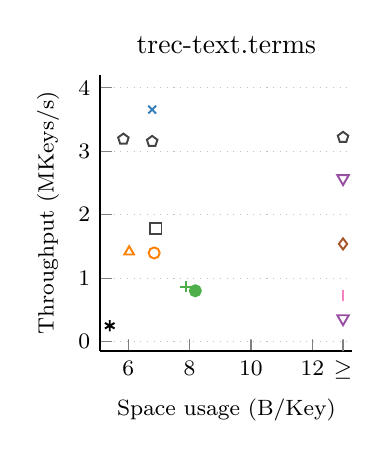
\begin{tikzpicture}
    \begin{axis}[
        title={trec-text.terms},
        plotCompetitorConstruction,
        legend to name=legendCompetitors,
      ]
      %% MULTIPLOT(name|ptitle|attr)
      %%   SELECT
      %%     MIN(bitsPerElement, 13) as x,
      %%     0.001*N/constructionTimeMilliseconds as y,
      %%     name,
      %%     attr,
      %%     paper_name AS ptitle
      %%   FROM competitors
      %%   JOIN competitorNames ON name = code_name
      %%   WHERE dataset="trec-text.terms"
      %%   ORDER BY name,x
      \addplot[mark=x,color=colorCentroidHollowTrie,solid] coordinates { (6.77934,3.65825) };
      \addlegendentry{Centroid Hollow Trie \cite{grossi2014decomposition}};
      \addplot[mark=o,color=colorDirectRankStoring,solid] coordinates { (6.84487,1.39791) };
      \addlegendentry{\textbf{Direct Rank Storing (20230130)}};
      \addplot[mark=triangle,color=colorDirectRankStoring,solid] coordinates { (6.02976,1.417) };
      \addlegendentry{\textbf{Direct Rank Storing (20230210)}};
      \addplot[mark=pentagon,color=colorHollowTrie,solid] coordinates { (5.84184,3.19176) (6.77952,3.15508) (13,3.21976) };
      \addlegendentry{Hollow Trie \cite{grossi2014decomposition}};
      \addplot[mark=asterisk,color=colorHollowTrieDist,solid] coordinates { (5.39703,0.25091) };
      \addlegendentry{Hollow Trie Dist (Java) \cite{belazzougui2011theoryPractice}};
      \addplot[mark=square,color=colorHollowTrie,solid] coordinates { (6.90449,1.78868) };
      \addlegendentry{Hollow Trie (Java) \cite{belazzougui2011theoryPractice}};
      \addplot[mark=diamond,color=colorLcp,solid] coordinates { (13,1.54032) };
      \addlegendentry{Lcp (Java) \cite{belazzougui2011theoryPractice}};
      \addplot[mark=+,color=colorPaCoTrieJava,solid] coordinates { (7.87968,0.861823) };
      \addlegendentry{PaCoTrie (Java) \cite{belazzougui2011theoryPractice}};
      \addplot[mark=flippedTriangle,color=colorPathDecomposedTrie,solid] coordinates { (13,2.573) (13,0.364003) };
      \addlegendentry{Path Decomposed Trie \cite{grossi2014decomposition}};
      \addplot[mark=|,color=colorVllcp,solid] coordinates { (13,0.734053) };
      \addlegendentry{VLLcp (Java) \cite{belazzougui2011theoryPractice}};
      \addplot[mark=*,color=colorPaCoTrieJava,solid] coordinates { (8.18601,0.801701) };
      \addlegendentry{VLPaCoTrie (Java) \cite{belazzougui2011theoryPractice}};
    \end{axis}
\end{tikzpicture}
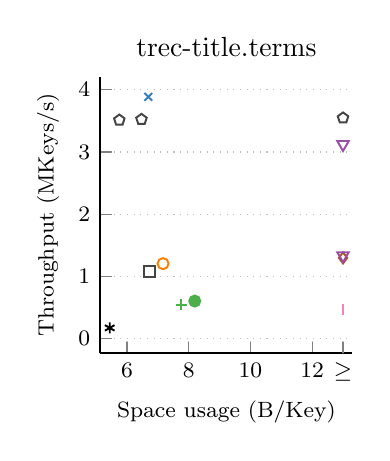
\begin{tikzpicture}
    \begin{axis}[
        title={trec-title.terms},
        plotCompetitorConstruction,
        legend to name=legendCompetitors,
      ]
      %% MULTIPLOT(name|ptitle|attr)
      %%   SELECT
      %%     MIN(bitsPerElement, 13) as x,
      %%     0.001*N/constructionTimeMilliseconds as y,
      %%     name,
      %%     attr,
      %%     paper_name AS ptitle
      %%   FROM competitors
      %%   JOIN competitorNames ON name = code_name
      %%   WHERE dataset="trec-title.terms"
      %%   ORDER BY name,x
      \addplot[mark=x,color=colorCentroidHollowTrie,solid] coordinates { (6.69053,3.88641) };
      \addlegendentry{Centroid Hollow Trie \cite{grossi2014decomposition}};
      \addplot[mark=o,color=colorDirectRankStoring,solid] coordinates { (7.16934,1.20304) };
      \addlegendentry{\textbf{Direct Rank Storing (20230130)}};
      \addplot[mark=pentagon,color=colorHollowTrie,solid] coordinates { (5.75304,3.51272) (6.4705,3.52402) (13,3.54683) };
      \addlegendentry{Hollow Trie \cite{grossi2014decomposition}};
      \addplot[mark=asterisk,color=colorHollowTrieDist,solid] coordinates { (5.44223,0.168949) };
      \addlegendentry{Hollow Trie Dist (Java) \cite{belazzougui2011theoryPractice}};
      \addplot[mark=square,color=colorHollowTrie,solid] coordinates { (6.73464,1.08084) };
      \addlegendentry{Hollow Trie (Java) \cite{belazzougui2011theoryPractice}};
      \addplot[mark=diamond,color=colorLcp,solid] coordinates { (13,1.29547) };
      \addlegendentry{Lcp (Java) \cite{belazzougui2011theoryPractice}};
      \addplot[mark=+,color=colorPaCoTrieJava,solid] coordinates { (7.76357,0.540952) };
      \addlegendentry{PaCoTrie (Java) \cite{belazzougui2011theoryPractice}};
      \addplot[mark=flippedTriangle,color=colorPathDecomposedTrie,solid] coordinates { (13,3.12242) (13,1.3333) };
      \addlegendentry{Path Decomposed Trie \cite{grossi2014decomposition}};
      \addplot[mark=|,color=colorVllcp,solid] coordinates { (13,0.46538) };
      \addlegendentry{VLLcp (Java) \cite{belazzougui2011theoryPractice}};
      \addplot[mark=*,color=colorPaCoTrieJava,solid] coordinates { (8.19657,0.60086) };
      \addlegendentry{VLPaCoTrie (Java) \cite{belazzougui2011theoryPractice}};
    \end{axis}
\end{tikzpicture}
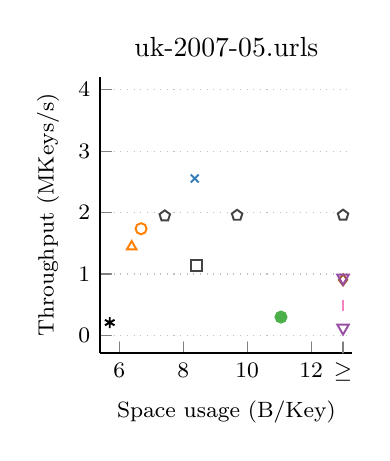
\begin{tikzpicture}
    \begin{axis}[
        title={uk-2007-05.urls},
        plotCompetitorConstruction,
        legend to name=legendCompetitors,
      ]
      %% MULTIPLOT(name|ptitle|attr)
      %%   SELECT
      %%     MIN(bitsPerElement, 13) as x,
      %%     0.001*N/constructionTimeMilliseconds as y,
      %%     name,
      %%     attr,
      %%     paper_name AS ptitle
      %%   FROM competitors
      %%   JOIN competitorNames ON name = code_name
      %%   WHERE dataset="uk-2007-05.urls"
      %%   ORDER BY name,x
      \addplot[mark=x,color=colorCentroidHollowTrie,solid] coordinates { (8.35901,2.55505) };
      \addlegendentry{Centroid Hollow Trie \cite{grossi2014decomposition}};
      \addplot[mark=o,color=colorDirectRankStoring,solid] coordinates { (6.67972,1.73689) };
      \addlegendentry{\textbf{Direct Rank Storing (20230130)}};
      \addplot[mark=triangle,color=colorDirectRankStoring,solid] coordinates { (6.38508,1.44618) };
      \addlegendentry{\textbf{Direct Rank Storing (20230210)}};
      \addplot[mark=pentagon,color=colorHollowTrie,solid] coordinates { (7.42151,1.94588) (9.68466,1.95569) (13,1.95778) };
      \addlegendentry{Hollow Trie \cite{grossi2014decomposition}};
      \addplot[mark=asterisk,color=colorHollowTrieDist,solid] coordinates { (5.69871,0.210187) };
      \addlegendentry{Hollow Trie Dist (Java) \cite{belazzougui2011theoryPractice}};
      \addplot[mark=square,color=colorHollowTrie,solid] coordinates { (8.40711,1.13878) };
      \addlegendentry{Hollow Trie (Java) \cite{belazzougui2011theoryPractice}};
      \addplot[mark=diamond,color=colorLcp,solid] coordinates { (13,0.905246) };
      \addlegendentry{Lcp (Java) \cite{belazzougui2011theoryPractice}};
      \addplot[mark=+,color=colorPaCoTrieJava,solid] coordinates { (11.0866,0.298624) };
      \addlegendentry{PaCoTrie (Java) \cite{belazzougui2011theoryPractice}};
      \addplot[mark=flippedTriangle,color=colorPathDecomposedTrie,solid] coordinates { (13,0.935498) (13,0.123092) };
      \addlegendentry{Path Decomposed Trie \cite{grossi2014decomposition}};
      \addplot[mark=|,color=colorVllcp,solid] coordinates { (13,0.480317) };
      \addlegendentry{VLLcp (Java) \cite{belazzougui2011theoryPractice}};
      \addplot[mark=*,color=colorPaCoTrieJava,solid] coordinates { (11.0581,0.29981) };
      \addlegendentry{VLPaCoTrie (Java) \cite{belazzougui2011theoryPractice}};
    \end{axis}
\end{tikzpicture}


    \begin{tikzpicture}
        \ref*{legendCompetitors}
    \end{tikzpicture}

    \caption{Construction throughput for different data sets.}
\end{figure}

\begin{figure}[H]
    \centering
    % IMPORT-DATA competitors data/competitors.txt
% IMPORT-DATA competitorNames data/__competitorNames.txt
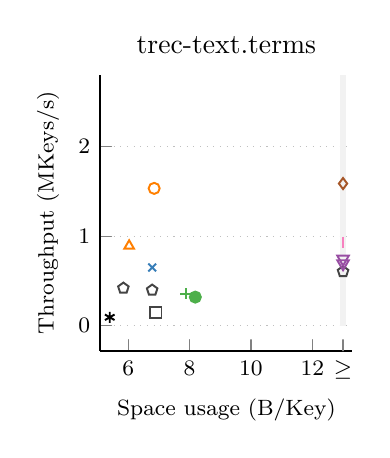
\begin{tikzpicture}
    \begin{axis}[
        title={trec-text.terms},
        plotCompetitorQueries,
        legend to name=legendCompetitorsQueries,
      ]
      \addplot[no marks,veryLightGrey,line width=2pt,forget plot,sharp plot] coordinates { (13,0) (13,100) };
      %% MULTIPLOT(name|ptitle|attr)
      %%   SELECT
      %%     MIN(bitsPerElement, 13) as x,
      %%     0.001*numQueries/queryTimeMilliseconds as y,
      %%     name,
      %%     attr,
      %%     name AS title,
      %%     paper_name AS ptitle
      %%   FROM competitors
      %%   JOIN competitorNames ON name = code_name
      %%   WHERE dataset="trec-text.terms"
      %%   ORDER BY name,x
      \addplot[mark=x,color=colorCentroidHollowTrie,solid] coordinates { (6.77934,0.650618) };
      \addlegendentry{Centroid Hollow Trie \cite{grossi2014decomposition}};
      \addplot[mark=o,color=colorDirectRankStoring,solid] coordinates { (6.84487,1.53492) };
      \addlegendentry{\textbf{Direct Rank Storing (20230130)}};
      \addplot[mark=triangle,color=colorDirectRankStoring,solid] coordinates { (6.02976,0.892857) };
      \addlegendentry{\textbf{Direct Rank Storing (20230210)}};
      \addplot[mark=pentagon,color=colorHollowTrie,solid] coordinates { (5.84184,0.42008) (6.77952,0.398248) (13,0.604595) };
      \addlegendentry{Hollow Trie \cite{grossi2014decomposition}};
      \addplot[mark=asterisk,color=colorHollowTrieDist,solid] coordinates { (5.39703,0.0941531) };
      \addlegendentry{Hollow Trie Dist (Java) \cite{belazzougui2011theoryPractice}};
      \addplot[mark=square,color=colorHollowTrie,solid] coordinates { (6.90449,0.150015) };
      \addlegendentry{Hollow Trie (Java) \cite{belazzougui2011theoryPractice}};
      \addplot[mark=diamond,color=colorLcp,solid] coordinates { (13,1.58856) };
      \addlegendentry{Lcp (Java) \cite{belazzougui2011theoryPractice}};
      \addplot[mark=+,color=colorPaCoTrieJava,solid] coordinates { (7.87968,0.358551) };
      \addlegendentry{PaCoTrie (Java) \cite{belazzougui2011theoryPractice}};
      \addplot[mark=flippedTriangle,color=colorPathDecomposedTrie,solid] coordinates { (13,0.745712) (13,0.694203) };
      \addlegendentry{Path Decomposed Trie \cite{grossi2014decomposition}};
      \addplot[mark=|,color=colorVllcp,solid] coordinates { (13,0.933707) };
      \addlegendentry{VLLcp (Java) \cite{belazzougui2011theoryPractice}};
      \addplot[mark=*,color=colorPaCoTrieJava,solid] coordinates { (8.18601,0.319693) };
      \addlegendentry{VLPaCoTrie (Java) \cite{belazzougui2011theoryPractice}};
    \end{axis}
\end{tikzpicture}
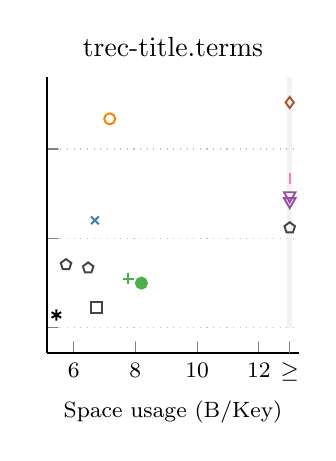
\begin{tikzpicture}
    \begin{axis}[
        title={trec-title.terms},
        plotCompetitorQueries,
        legend to name=legendCompetitorsQueries,ylabel={},yticklabels={,,}
      ]
      \addplot[no marks,veryLightGrey,line width=2pt,forget plot,sharp plot] coordinates { (13,0) (13,100) };
      %% MULTIPLOT(name|ptitle|attr)
      %%   SELECT
      %%     MIN(bitsPerElement, 13) as x,
      %%     0.001*numQueries/queryTimeMilliseconds as y,
      %%     name,
      %%     attr,
      %%     name AS title,
      %%     paper_name AS ptitle
      %%   FROM competitors
      %%   JOIN competitorNames ON name = code_name
      %%   WHERE dataset="trec-title.terms"
      %%   ORDER BY name,x
      \addplot[mark=x,color=colorCentroidHollowTrie,solid] coordinates { (6.69053,1.20192) };
      \addlegendentry{Centroid Hollow Trie \cite{grossi2014decomposition}};
      \addplot[mark=o,color=colorDirectRankStoring,solid] coordinates { (7.16934,2.33645) };
      \addlegendentry{\textbf{Direct Rank Storing (20230130)}};
      \addplot[mark=pentagon,color=colorHollowTrie,solid] coordinates { (5.75304,0.707214) (6.4705,0.670241) (13,1.11857) };
      \addlegendentry{Hollow Trie \cite{grossi2014decomposition}};
      \addplot[mark=asterisk,color=colorHollowTrieDist,solid] coordinates { (5.44223,0.144592) };
      \addlegendentry{Hollow Trie Dist (Java) \cite{belazzougui2011theoryPractice}};
      \addplot[mark=square,color=colorHollowTrie,solid] coordinates { (6.73464,0.225175) };
      \addlegendentry{Hollow Trie (Java) \cite{belazzougui2011theoryPractice}};
      \addplot[mark=diamond,color=colorLcp,solid] coordinates { (13,2.51889) };
      \addlegendentry{Lcp (Java) \cite{belazzougui2011theoryPractice}};
      \addplot[mark=+,color=colorPaCoTrieJava,solid] coordinates { (7.76357,0.551268) };
      \addlegendentry{PaCoTrie (Java) \cite{belazzougui2011theoryPractice}};
      \addplot[mark=flippedTriangle,color=colorPathDecomposedTrie,solid] coordinates { (13,1.47929) (13,1.41343) };
      \addlegendentry{Path Decomposed Trie \cite{grossi2014decomposition}};
      \addplot[mark=|,color=colorVllcp,solid] coordinates { (13,1.67224) };
      \addlegendentry{VLLcp (Java) \cite{belazzougui2011theoryPractice}};
      \addplot[mark=*,color=colorPaCoTrieJava,solid] coordinates { (8.19657,0.500501) };
      \addlegendentry{VLPaCoTrie (Java) \cite{belazzougui2011theoryPractice}};
    \end{axis}
\end{tikzpicture}
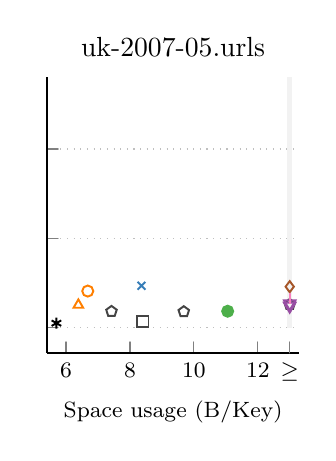
\begin{tikzpicture}
    \begin{axis}[
        title={uk-2007-05.urls},
        plotCompetitorQueries,
        legend to name=legendCompetitorsQueries,ylabel={},yticklabels={,,}
      ]
      \addplot[no marks,veryLightGrey,line width=2pt,forget plot,sharp plot] coordinates { (13,0) (13,100) };
      %% MULTIPLOT(name|ptitle|attr)
      %%   SELECT
      %%     MIN(bitsPerElement, 13) as x,
      %%     0.001*numQueries/queryTimeMilliseconds as y,
      %%     name,
      %%     attr,
      %%     name AS title,
      %%     paper_name AS ptitle
      %%   FROM competitors
      %%   JOIN competitorNames ON name = code_name
      %%   WHERE dataset="uk-2007-05.urls"
      %%   ORDER BY name,x
      \addplot[mark=x,color=colorCentroidHollowTrie,solid] coordinates { (8.35901,0.471143) };
      \addlegendentry{Centroid Hollow Trie \cite{grossi2014decomposition}};
      \addplot[mark=o,color=colorDirectRankStoring,solid] coordinates { (6.67972,0.411692) };
      \addlegendentry{\textbf{Direct Rank Storing (20230130)}};
      \addplot[mark=triangle,color=colorDirectRankStoring,solid] coordinates { (6.38508,0.25641) };
      \addlegendentry{\textbf{Direct Rank Storing (20230210)}};
      \addplot[mark=pentagon,color=colorHollowTrie,solid] coordinates { (7.42151,0.183857) (9.68466,0.180848) (13,0.261097) };
      \addlegendentry{Hollow Trie \cite{grossi2014decomposition}};
      \addplot[mark=asterisk,color=colorHollowTrieDist,solid] coordinates { (5.69871,0.0531675) };
      \addlegendentry{Hollow Trie Dist (Java) \cite{belazzougui2011theoryPractice}};
      \addplot[mark=square,color=colorHollowTrie,solid] coordinates { (8.40711,0.0706614) };
      \addlegendentry{Hollow Trie (Java) \cite{belazzougui2011theoryPractice}};
      \addplot[mark=diamond,color=colorLcp,solid] coordinates { (13,0.460723) };
      \addlegendentry{Lcp (Java) \cite{belazzougui2011theoryPractice}};
      \addplot[mark=+,color=colorPaCoTrieJava,solid] coordinates { (11.0866,0.185856) };
      \addlegendentry{PaCoTrie (Java) \cite{belazzougui2011theoryPractice}};
      \addplot[mark=flippedTriangle,color=colorPathDecomposedTrie,solid] coordinates { (13,0.271186) (13,0.244708) };
      \addlegendentry{Path Decomposed Trie \cite{grossi2014decomposition}};
      \addplot[mark=|,color=colorVllcp,solid] coordinates { (13,0.323992) };
      \addlegendentry{VLLcp (Java) \cite{belazzougui2011theoryPractice}};
      \addplot[mark=*,color=colorPaCoTrieJava,solid] coordinates { (11.0581,0.186376) };
      \addlegendentry{VLPaCoTrie (Java) \cite{belazzougui2011theoryPractice}};
    \end{axis}
\end{tikzpicture}


    \begin{tikzpicture}
        \ref*{legendCompetitors}
    \end{tikzpicture}

    \caption{Query throughput for different data sets.}
\end{figure}

\bibliographystyle{plainurl}
\bibliography{plots}

\end{document}
